\documentclass[11pt]{article}
\usepackage[utf8]{inputenc}
\usepackage{graphicx}
\usepackage[T1]{fontenc}
\usepackage{listings}
\usepackage{amsmath}
\usepackage{lscape}
\usepackage{bm}
    \usepackage[margin=1.2in]{geometry}
%\usepackage[section]{placeins} %prevents figs appearing before the start of the section in which it appears

\title{Supplementary Materials}
\author{Joe Challenger \& Tom Churcher}
%\date{February 2020}

\begin{document}

\maketitle

\section*{A brief intro to R}
To do. How to load libraries, define a comment, etc.

\section{Loading \& summarising a dataset}

In this document, we will demonstrate how to carry out the statistical analyses discussed in the main manuscript. To demonstrate these concepts, we will use a simulated dataset. This dataset has been uploaded with these materials, along with an R script containing the work outlined in this Supplementary file. To run the R script you should download R (link) \& RStudio (link). If you wish to run the script, you should download the ZIP file, and extract the folder. Then, double-click on the project file `XXX.Rproj' to open it in RStudio.

Once the project file has been opened, you can then open the R script called `YYY'. The dataset has been stored as an .rds file, and can be loaded using the following command:
%{\tt
\begin{verbatim}
> df <- readRDS(`data_for_plot.rds')
\end{verbatim}
%}
Let's take a look at the data:
\begin{verbatim}
> dim(df)
[1] 343  10
> head(df)
  day hut sleeper treatment total unf_live unf_dead bf_live bf_dead tot_dead
1   1   1       2         C     4        2        0       2       0        0
2   1   2       3       N1u     7        7        0       0       0        0
3   1   3       4       N1w    12        9        1       2       0        1
4   1   4       5       N2u     5        4        1       0       0        1
5   1   5       6       N2w    10        8        0       2       0        0
6   1   6       7       N3u     2        2        0       0       0        0
\end{verbatim}
For this experimental hut trial (EHT), 343 data points were collected. For each of these, the total number of mosquitoes entering each hut each night was recorded, as well as their mortality \& blood-feeding status (\verb+unf_live+ = unfed \& alive; \verb+unf_dead+ = unfed \& dead; \verb+bf_live+ = blood fed \& live; \verb+bf_dead+ = blood fed \& dead). As the following commands tell us, the trial contained 7 different nets, 7 volunteers, and 7 huts:
\begin{verbatim}
> table(df$treatment)

  C N1u N1w N2u N2w N3u N3w 
 49  49  49  49  49  49  49 
> table(df$hut)

 1  2  3  4  5  6  7 
49 49 49 49 49 49 49 
> table(df$sleeper)

 1  2  3  4  5  6  7 
49 49 49 49 49 49 49 
\end{verbatim}
This EHT contains an untreated net (labelled `C' for control) and three insecticide-treated nets (ITNs), labelled \verb+N1+, \verb+N2+ and \verb+N3+. The suffix `u' indicates an unwashed (\textit{i.e.} new) ITN; the suffix `w' indicates a washed (\textit{i.e.} aged) ITN.

\section{Visualising the EHT data}

Figure~1 shows some output from 3-arms of the simulated trial, namely the untreated control, and both unwashed and washed \verb+N1+ nets. The R code that accompanies this document shows how these panels may be generated.

\begin{landscape}
\begin{figure}%[p]
\centering
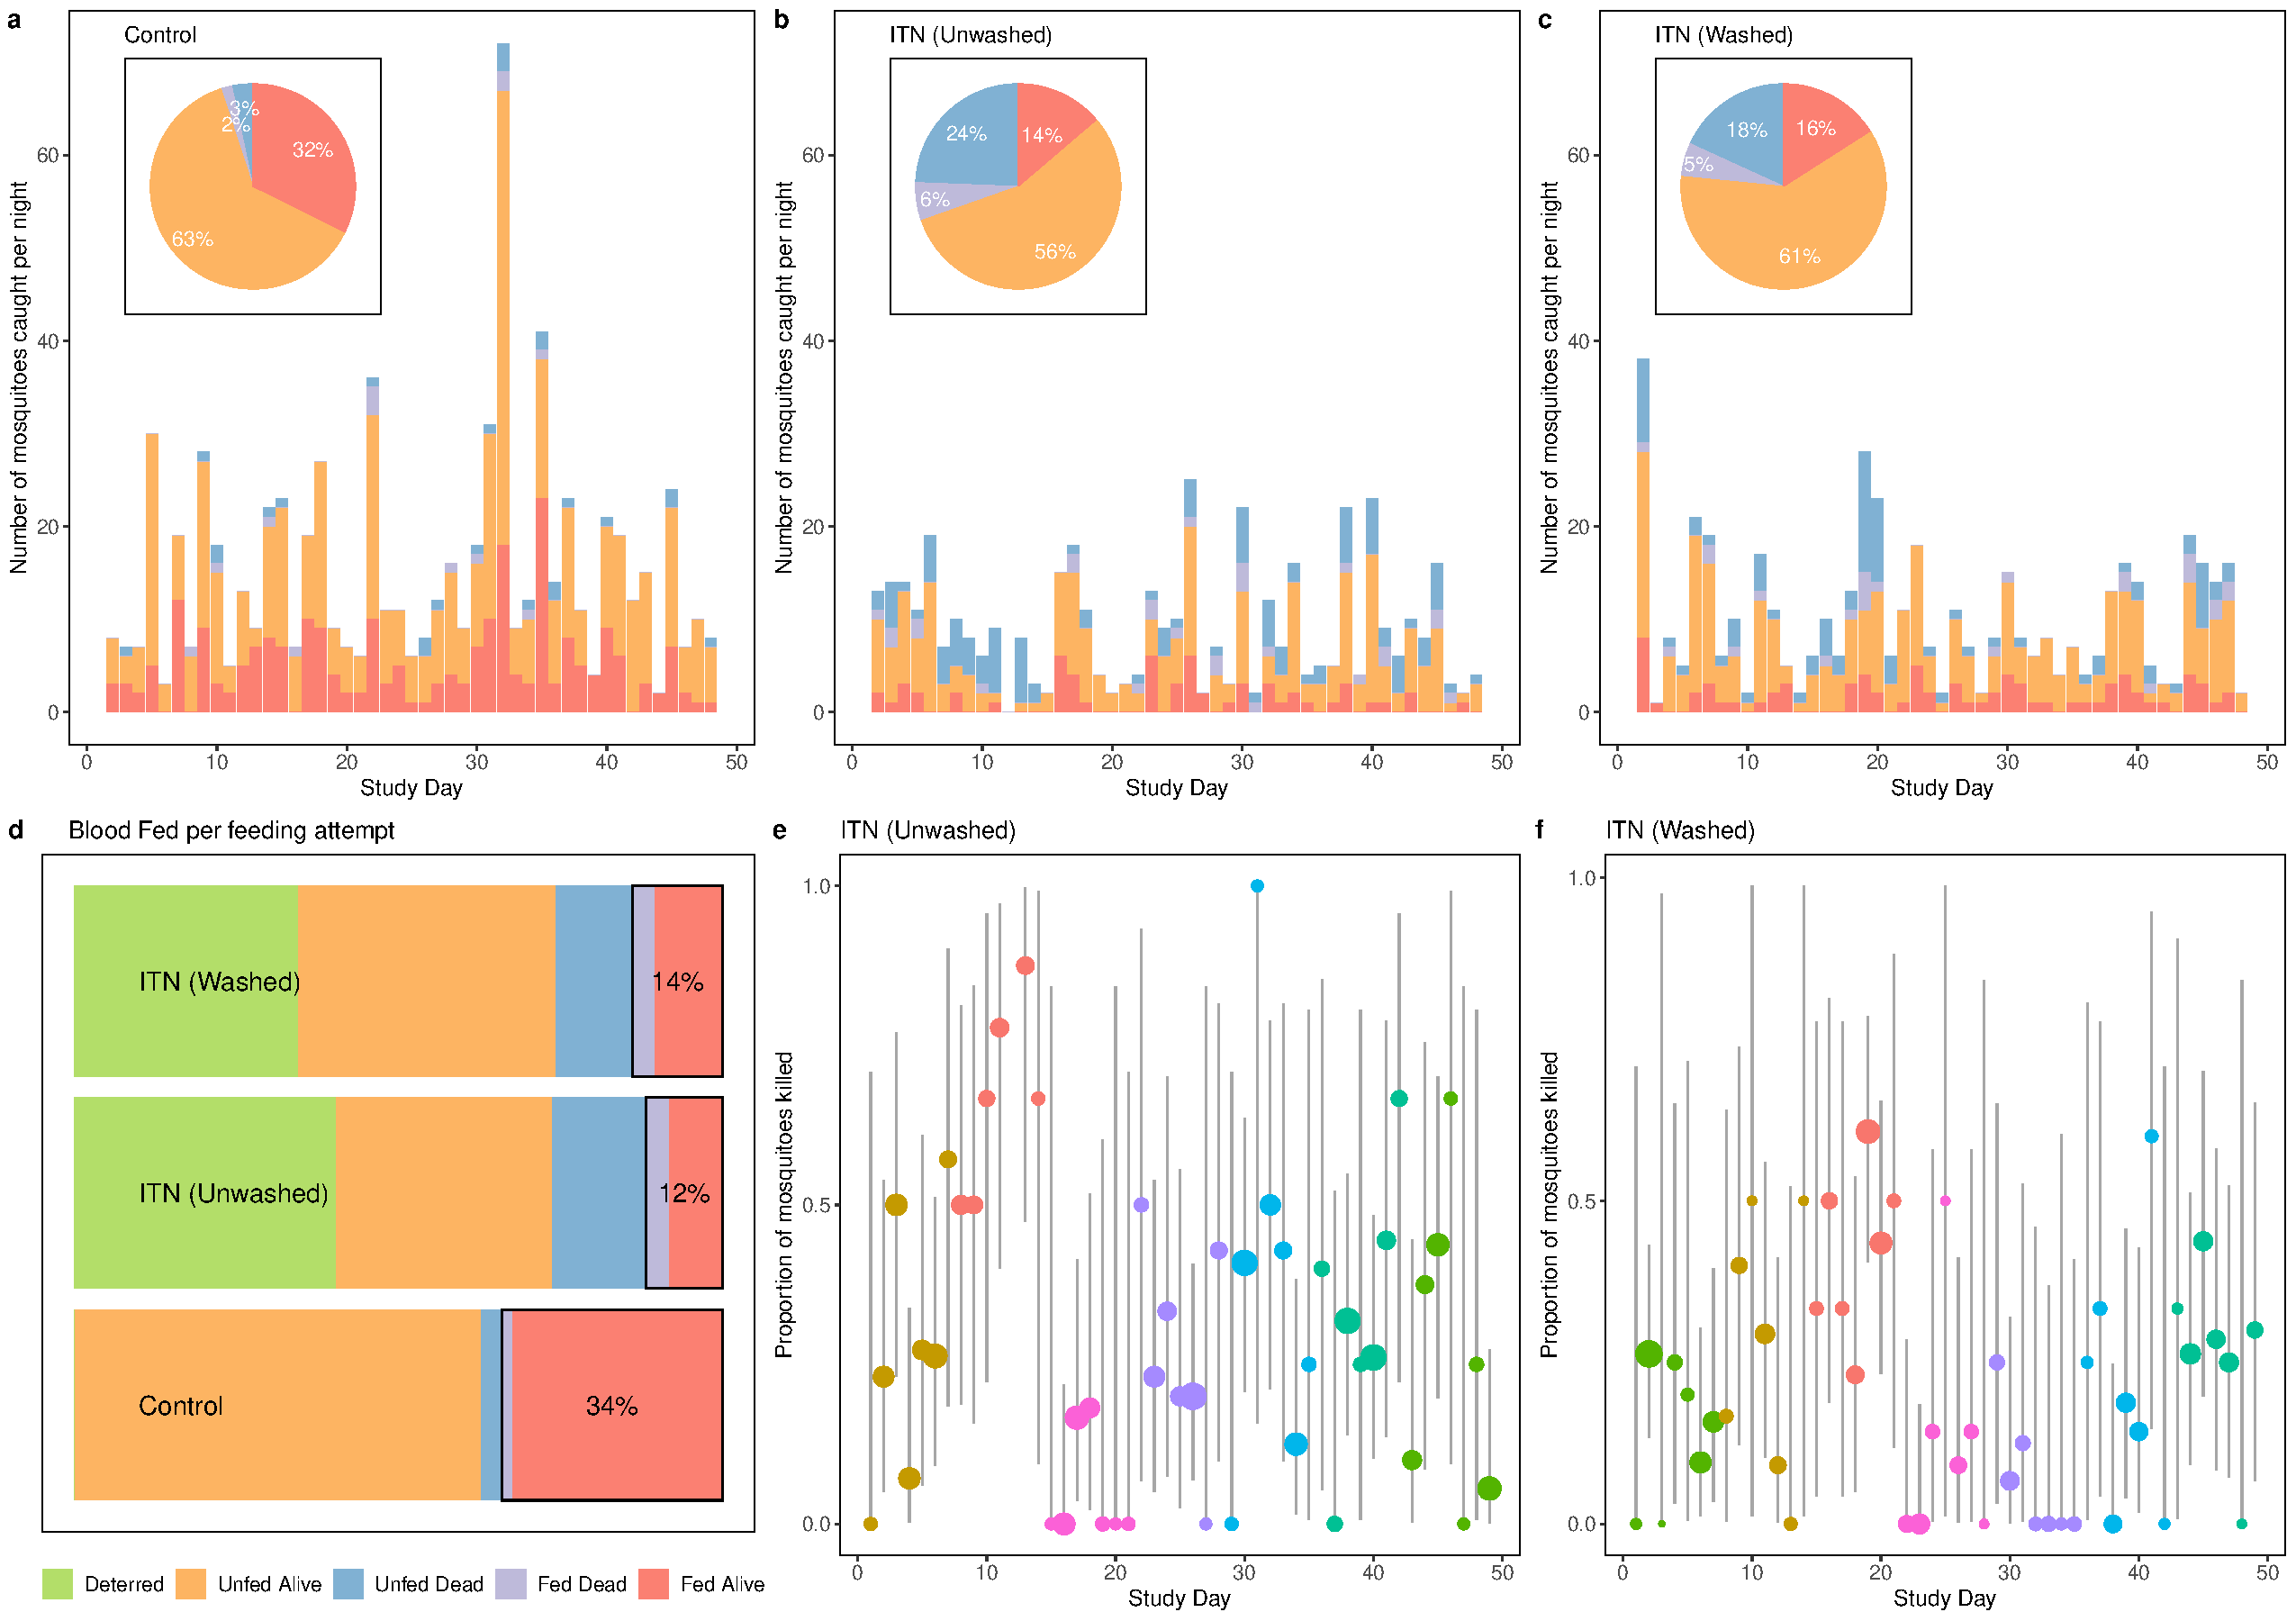
\includegraphics[scale=0.47]{Six_panel_figure.pdf}
\caption{Visualisation of the simulated EHT data. Here we show output from 3-arms of the simulated trial, namely the untreated control, and both unwashed and washed N1 nets}
%\label{fig:EIR50}
\end{figure}
\end{landscape}

\section{Fitting a regression model to the data}

We'll now show how to fit the regression model shown in Equation~1 in the main text. As this model contains an observation-level random effect, we first need to provide a unique indicator variable for each row in the data frame \textit{e.g.}
\begin{verbatim} 
df$observation <- factor(formatC(1:nrow(df), flag="0", width=3)) 
\end{verbatim}%change up?
For mortality, we
\begin{verbatim} 
fit <-
  glmer(
    cbind(tot_dead, total - tot_dead) ~
      treatment + (1 | hut) + (1 | sleeper) + (1 | observation),
    family = binomial, data = df)
\end{verbatim} 
This is equivalent to the equation we wrote down in the main text, which we also include here, for convenience:
\begin{equation}
\log \left( \frac{p_{ijk}}{1-p_{ijk}} \right) = \beta_0 + \sum_{m}\beta_m + b_i + h_j + v_k.
\end{equation}
Here we characeterise each data point using the subscripts $(i,j,k)$. Subscript $i$ uniquely identifies each data point, $j$ indicates the hut used, $k$ indicates the volunteer sleeping under the net.
Then we run the command \verb+summary(fit)+ to examine the fitted model. This output is quite lengthy: here we will focus on the fixed and random effects. The former will look like this:
\begin{verbatim} 
Fixed effects:
             Estimate Std. Error z value Pr(>|z|)    
(Intercept)   -3.2998     0.2760 -11.957  < 2e-16 ***
treatmentN1u   2.3942     0.2369  10.107  < 2e-16 ***
treatmentN1w   1.6820     0.2408   6.985 2.85e-12 ***
treatmentN2u   2.0851     0.2379   8.764  < 2e-16 ***
treatmentN2w   1.6310     0.2387   6.832 8.37e-12 ***
treatmentN3u   2.4207     0.2375  10.191  < 2e-16 ***
treatmentN3w   1.7341     0.2376   7.298 2.93e-13 ***
\end{verbatim} 
An estimate for each of the fixed effects is provided, along with its standard error, which indicates the level of precision with which each parameter has been estimated. The z \& p values relate to testing whether the parameter estimates are significantly different from 0. It is not immediately obvious how these parameter values relate to our problem: working out the proportion of mosquitoes killed (or blood fed) in each trial arm. This is because a binomial regression like this has been carried out by transforming the proportions onto the log-odds scale. This transformation maps the interval [0,1] (used for proportions, prevalence, or probabilities) to the interval $[-\infty, \infty]$. This removes the difficulty caused by the fact that the probability scale (which runs from 0 to 1) has a floor and ceiling \textit{i.e.} values below 0 and above 1 are forbidden.

The estimated values of the random effects will be presented like this:
\begin{verbatim} 
Random effects:
 Groups      Name        Variance Std.Dev.
 observation (Intercept) 0.2406   0.4905  
 sleeper     (Intercept) 0.1529   0.3910  
 hut         (Intercept) 0.1103   0.3321  
Number of obs: 343, groups:  observation, 343; sleeper, 7; hut, 7
\end{verbatim} 
By definition, all the random effects are normally distributed with zero mean. Therefore, they are fully characterised by the values of the variance (or, equivalently, the standard deviation).

In order to understand the output of the regression model, we will use the inverse of this log-odds transformation. If $X(p)$ denotes the log-odds-transformed proportion, we write
\[
X(p) = \log \left( \frac{p}{1-p} \right).
\]
Note that, on the log-odds scale, values can be positive or negative. A value of 0 corresponds to $p=0.5$. We can write the inverse function like this:
\[
p = \textrm{InvLogit}(X) = \frac{\exp(X)}{\exp(X) + 1}
\]
Figure~2 shows this function, which approaches 1 as $X\to\infty$, and approaches 0 as $X\to-\infty$. In R, we will define a function to carry out this transformation, as we will be using it frequently. We write
\begin{verbatim} 
InvLogit <- function(X){
  exp(X)/(1+exp(X))
}
\end{verbatim} 
Let's use this function to find the mortality in the control arm (where untreated nets were used). This is indicated by the intercept in the regression model. 
\begin{verbatim} 
InvLogit(coef(summary(fit))["(Intercept)", "Estimate"])
0.03557956
\end{verbatim} 
Furthermore, we can use the standard error to create a 95\% confidence interval. We do this by adding or subtracting $1.96\times$ the standard error, before converting to a probability: 
\begin{verbatim} 
InvLogit(coef(summary(fit))["(Intercept)", "Estimate"]+
c(-1,1)*1.96*coef(summary(fit))["(Intercept)", "Std. Error"])
[1] 0.2025497 0.3915961
\end{verbatim} 
Let's now estimate the mortality in one of the arms containing an ITN. To find the estimated mortality due to unwashed `N1' nets we perform this calcualation:
\begin{verbatim} 
InvLogit(coef(summary(fit))["(Intercept)", "Estimate"] +
coef(summary(fit))["treatmentN1u", "Estimate"])
[1] 0.2879172
\end{verbatim} 
This follows from Eq, 1: we have to add the value of the fixed effect parameter to the intercept ($\beta_0$) before applying the transformation to the probability scale. We can also generate confidence intervals for this estimated mortality. Strictly speaking we should use the standard errors of both parameter estimates here, and respect the fact that they may be correlated with each other. The variance-covariance matrix for the fixed-effects parameters can be accessed with the \verb+vcov()+ function. To calculate the mortality of the unwashed N1 ITN, we had to add together two regression parameters. We can use the standard errors to calculate the standard error in their sum (using results for normally-distributed random variables).
\begin{verbatim}
rho1_2 <- vcov(fit)[1,2]/(sqrt(vcov(fit)[1,1])*sqrt(vcov(fit)[2,2]))
sigma1_2 <-  sqrt(vcov(fit)[1,1] + vcov(fit)[2,2] + 
                 2 * rho1_2 *(sqrt(vcov(fit)[1,1]) *(sqrt(vcov(fit)[2,2]))))
\end{verbatim}


For some analyses, we will want to group washed \& unwashed nets of the same type together. We do this by introducing a new variable `net'.
\begin{verbatim}
> df$net <- NA
> df[df$treatment==`C',]$net <- `C'
> df[df$treatment==`N1u',]$net <- `N1'
> df[df$treatment==`N1w',]$net <- `N1'
> df[df$treatment==`N2u',]$net <- `N2'
> df[df$treatment==`N2w',]$net <- `N2'
> df[df$treatment==`N3u',]$net <- `N3'
> df[df$treatment==`N3w',]$net <- `N3'
> table(df$net, useNA = 'a')

   C   N1   N2   N3 <NA> 
  49   98   98   98    0 
\end{verbatim}

We can then fit this model like this:
\begin{verbatim}
> fit_n <-
+   glmer(
+     cbind(tot_dead, total - tot_dead) ~
+       net + (1 | hut) + (1 | sleeper) + (1 | observation),
+     family = binomial, data = df) 
\end{verbatim}

\begin{figure}%[p]
\centering
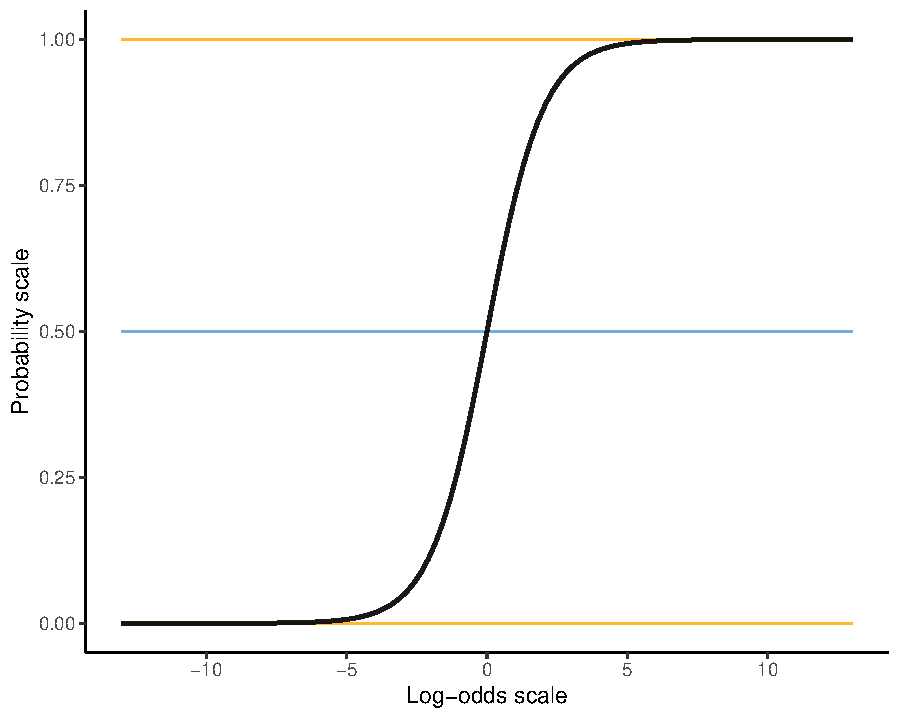
\includegraphics[scale=0.8]{logit_plot.pdf}
\caption{Relationship between the log-odds and probabilty scales. The function is symmetric about 0, which corresponds to a probability of 0.5. The probability approaches 1 as the log-odds value becomes very large (technically, we say `as it tends to infinity'). Similarly, the probability goes to 0 as the log-odds value tends to minus infinity.}
%\label{fig:EIR50}
\end{figure}


\section{Deterrence}

In EHTs, it is often observed that fewer mosquitoes are collected in huts containing ITNs, compared to those containing untreated nets. This phenomenon is known as `deterrence'. We can examine whether or not this is the case for our dataset by calculating the mean number of mosquitoes observed across all the different trial arms:
\begin{verbatim}
tapply(df$total, df$treatment, mean)
        C       N1u       N1w       N2u       N2w       N3u       N3w 
16.387755  9.714286 10.836735 10.061224 11.102041  8.469388 12.653061 
\end{verbatim}
In this EHT, it appears that fewer mosquitoes entered huts containing ITNs, compared with those containing the untreated nets. 
We will use a different type of regression model to examine this. This is because we will be dealing with mosquito count data, rather than looking at proportions (\textit{e.g.} proportion of mosquitoes killed or blood fed). Count data can be analysed by using a Poisson distribution, or a two-parameter distribution, such as the negative binomial. The latter is used when the count data are \textit{overdispersed}, \textit{i.e.} the standard deviation of the data is greater than its mean value. It is possible to perform a statistical test (\textit{include here?}), to see which distribution to use. However, in our experience with EHT trials, the data are almost always overdipsersed. Therefore, we will use the negative binomial distribution in this document. We perform a negative binomial regression using the function \verb+glmer.nb()+, also from the \verb+lme4+ package.
\begin{verbatim}
fit_nb <- glmer.nb(total ~ treatment + (1|sleeper), data = df)
summary(fit_nb)
\end{verbatim}
(Note that here we've dropped the random-effect for `hut', as it produced a singular model fit, with a estimated variance very close to 0. We'll discuss this in more detail in a later section). Let's look at the (truncated) model output:
\begin{verbatim}
Random effects:
 Groups  Name        Variance Std.Dev.
 sleeper (Intercept) 0.001653 0.04066 
Number of obs: 343, groups:  sleeper, 7

Fixed effects:
             Estimate Std. Error z value Pr(>|z|)    
(Intercept)    2.7935     0.1084  25.771  < 2e-16 ***
treatmentN1u  -0.5198     0.1541  -3.372 0.000745 ***
treatmentN1w  -0.4119     0.1531  -2.691 0.007124 ** 
treatmentN2u  -0.4869     0.1534  -3.173 0.001509 ** 
treatmentN2w  -0.3887     0.1528  -2.544 0.010971 *  
treatmentN3u  -0.6576     0.1549  -4.244  2.2e-05 ***
treatmentN3w  -0.2563     0.1523  -1.683 0.092410 .  
\end{verbatim}
Note that all the fixed-effect parameters are negative, since fewer mosquitoes enter huts containing an ITN, relative to the control. To understand the numerical values presented here, we must appreciate that the counts have been log-transformed. If we take the exponential of the intercept we find:
\begin{verbatim}
exp(coef(summary(fit_nb))["(Intercept)", "Estimate"])
[1] 16.33775
\end{verbatim}
This value is extremely close to the mean mosquito count found in the control arm (see above). The regression model will also return an estimate of the dispersion parameter:
\begin{verbatim}
getME(fit_nb, "glmer.nb.theta")
[1] 2.015564
\end{verbatim}
Let's now calculate the mean number of mosquitoes per night in huts contained unwashed N1 nets:
\begin{verbatim}
exp(coef(summary(fit_nb))["(Intercept)", "Estimate"]+
coef(summary(fit_nb))["treatmentN1u", "Estimate"])
[1] 9.714779
\end{verbatim}
We can use these values to estimate the deterrence effect in terms of a percentage:
\begin{verbatim}
mean_C <- exp(coef(summary(fit_nb))["(Intercept)", "Estimate"])
mean_E1 <- exp(coef(summary(fit_nb))["(Intercept)", "Estimate"]+
100*(1-mean_E1/mean_C)
[1] 40.53786
\end{verbatim}

\section{Superiority trials}

Frequently in EHTs, we are interesting in seeing if one type of bednet is superior to another, in terms of \textit{e.g.} mosquito mortality or blood-feeding inhibition. This could be a comparison between an ITN and the untreated control, or a comparison between two ITNs. When the logistic regression model is fitted in lme4, a p value for a Wald Z-test is returned, along with the estimates of the value of each fixed effect. This p value stems from a null hypothesis that the value of the fixed effect is 0 (or, alternatively, the mortality odds ratio for a particular ITN relative to the untreated control is equal to 1). Let's recap the output for the fixed-effect parameters shown in the previous section:
\begin{verbatim}
Fixed effects:
             Estimate Std. Error z value Pr(>|z|)    
(Intercept)    2.7935     0.1084  25.771  < 2e-16 ***
treatmentN1u  -0.5198     0.1541  -3.372 0.000745 ***
treatmentN1w  -0.4119     0.1531  -2.691 0.007124 ** 
treatmentN2u  -0.4869     0.1534  -3.173 0.001509 ** 
treatmentN2w  -0.3887     0.1528  -2.544 0.010971 *  
treatmentN3u  -0.6576     0.1549  -4.244  2.2e-05 ***
treatmentN3w  -0.2563     0.1523  -1.683 0.092410 .  
\end{verbatim}
Here we can see whether differences in mortality between the untreated control and any of the ITNs are judged to be significant. However, it is not immediately obvious how to test for superiority of one ITN compared to another. The simplest way to proceed is to change which net is chosen as the intercept in the regression model. By default, \verb+lme4+ will choose the first value, ordering the options alphabetically. One way to change the trial arm used for the intercept is to rename one of the treatment arms, so that it becomes the first category e.g. \verb+df[df$treatment=='N1u',]$treatment <- 'A'+. However, it would be better to avoid this, as re-labelling the trial arms can introduce confusion. One way forward is to make treatment a factor variable in R, and modify the order of the levels in the factor 
\begin{verbatim}
df$treatment <- as.factor(df$treatment)
#check the current levels of the factor
levels(df$treatment)
#Make unwashed N1 nets the intercept category
df$treatment <- relevel(df$treatment,"N1u") 
#check the levels again
levels(df$treatment)
\end{verbatim}
Once this has been carried out, we can run the regression analysis again, and find the desired p value. \textit{To do: actually show this- and also state that the fixed-effect has to be positive for superiority: if it's negative \& significant this means it's inferior!!}


\section{Non-inferiority trials}

In this section, we show how to use the output of the regression model to make an assessment of whether one ITN is non-inferior to another (\textit{e.g.} in terms of mosquito mortality or blood-feeding inhibition). In order to do this, a non-inferiority margin (NIM) must be selected. This should be chosen before the trial is started. According to World Health Organisation guidelines, the non-inferiority assessment should be made based on the odds ratio of the two products, and a NIM of 0.7 should be used for mosquito mortality (1.43 for blood-feeding inhibition). As with superiority trials, it is more straightforward if the comparator net is the reference category in the regression model. Let's test whether the ITN N3 is non-inferior to N2. We will use the \verb+net+ variable we defined earlier for this. In other words, we are comparing the mortality averaged across washed and unwashed nets of the same type. (Note: this should only be done if there are an equal number of data points in the washed and unwashed arms. Otherwise, the two arms will be unfairly weighted.) Let's ensure that the \verb+net+ variable is a factor variable and make N2 the default category (\textit{i.e.} the intercept).
\begin{verbatim}
df$net <- as.factor(df$net)
#check the levels
levels(df$net)
#relevel
df$net <- relevel(df$net,"N2") 
#check the levels again
levels(df$net)
\end{verbatim}
Now, if we run the regression model, the output for the fixed-effects should look like this:
\begin{verbatim}
Fixed effects:
            Estimate Std. Error z value Pr(>|z|)    
(Intercept)  -1.4751     0.2259  -6.529 6.64e-11 ***
netC         -1.8734     0.2297  -8.155 3.48e-16 ***
netN1         0.1882     0.1511   1.246    0.213    
netN3         0.2124     0.1508   1.409    0.159    
\end{verbatim}
The odds ratio of the mortality induced by N3 compared to N2 is:
\begin{verbatim}
exp(coef(summary(fit_n))['netN3','Estimate'])
[1] 1.236661
\end{verbatim}
Then, we use the standard error to find the 95\% confidence intervals
\begin{verbatim}
> exp(coef(summary(fit_n))['netN3','Estimate'] -
1.96*coef(summary(fit_n))['netN3','Std. Error'])
[1] 0.920288
> exp(coef(summary(fit_n))['netN3','Estimate'] +
1.96*coef(summary(fit_n))['netN3','Std. Error'])
[1] 1.661796
\end{verbatim}
We note that this interval lies entirely above the NIM. This means that we can say that N3 is non-inferior to N2, in terms of mosquito mortality.

\section{Simulate trials to aid power calculations}

Before carrying out an EHT, we should consider whether the trial is well-powered to answer the research question that is under consideration. Let's consider an example, where an EHT will be carried out to assess whether or not a novel ITN (`E2') is superior to a standard pyrethroid-only product (`E1'). We can use simulation-based methods to generate an estimate of trial power. When we simulate trials, we can select the average mortality induced by the ITNs. Let's imagine that we expect the pyrethroid-only net to kill 30\% of mosquitoes (this value could be estimated from previous studies in the same region, or a different region with a similar level of pyrethroid resistance in the wild mosquito population). We may be unsure what mortality to expect in our novel product, but we could pose the question: what would be the smallest improvement that would be worth measuring? If this is a difference of 10\%, we set the mortality of the novel ITN to be 40\%. The next step is, for the proposed trial design, is to simulate the trial and see if the new net is judged to be superior to the pyrethroid-only ITN. As the simulation will be random, it is necessary to simulate many trials (say 500 or 1000), and calculate the proportion of trials for which a verdict of superiority is reached. This will form our power estimate.

Our work builds on a paper by Johnston et al., published in \textit{Methods in Ecology and Evolution} in 2015 (\verb+doi:10.1111/2041-210X.12306+). In that article, the authors presented a tool (which is written as a function in R) which can simulate a range of GLMMs, including the logistic regression models considered here. We will utilise their R function \verb+simm.glmm+, to simulate an EHT. But first we must specify the trial design in R. Here we describe a seven-arm trial, containing 7 nets: an untreated control (``C") and 6 ITNs. Following Johnston \textit{et al.} we rotate the nets around the huts each week:
\begin{verbatim}
latsq <-
  rbind(
    c("C", "E1", "E2", "E3", "E4", "E5", "E6"),
    c("E6", "C", "E1", "E2", "E3", "E4", "E5"),
    c("E5", "E6", "C", "E1", "E2", "E3", "E4"),
    c("E4", "E5", "E6", "C", "E1", "E2", "E3"),
    c("E3", "E4", "E5", "E6", "C", "E1", "E2"),
    c("E2", "E3", "E4", "E5", "E6", "C", "E1"),
    c("E1", "E2", "E3", "E4", "E5", "E6", "C"))

colnames(latsq) <- paste("hut", 1:nrow(latsq), sep = "")
rownames(latsq) <- paste("week", 1:ncol(latsq), sep = "")
latsq
      hut1 hut2 hut3 hut4 hut5 hut6 hut7
week1 "C"  "E1" "E2" "E3" "E4" "E5" "E6"
week2 "E6" "C"  "E1" "E2" "E3" "E4" "E5"
week3 "E5" "E6" "C"  "E1" "E2" "E3" "E4"
week4 "E4" "E5" "E6" "C"  "E1" "E2" "E3"
week5 "E3" "E4" "E5" "E6" "C"  "E1" "E2"
week6 "E2" "E3" "E4" "E5" "E6" "C"  "E1"
week7 "E1" "E2" "E3" "E4" "E5" "E6" "C" 
\end{verbatim}
Now we make a data frame, in which we'll store the data:
\begin{verbatim}
mosdata <-
  expand.grid(
  hut = factor(1:ncol(latsq)),
  week = factor(1:nrow(latsq)),
  night = factor(1:7)
  )
mosdata <- mosdata[order(mosdata$hut, mosdata$week, mosdata$night),]

mosdata$net <- factor(diag(latsq[mosdata$week, mosdata$hut]))
\end{verbatim}
And we also need to specify where the volunteers will sleep each night.
\begin{verbatim}
aux <- rep(0,49) #enough data pts for a week
for(k in 1:7){ #Move the volunteers each night
  aux[(7*(k-1)+1):(7*(k-1)+7)] <- c( k : 7 , seq_len(k-1)  ) 
}
#repeat for all 7 weeks
mosdata$sleeper <- factor(rep(aux,7))
#Summarise data
table(mosdata$hut)
table(mosdata$net)
table(mosdata$sleeper)
\end{verbatim}
Run the command \verb+View(mosdata)+ to take a look at the full dataset. We now add an identifier for each observation. We'll also define a variable \verb+n+, for the number of mosquitoes entering each hut each night:
\begin{verbatim}
mosdata$observation <- factor(formatC(1:nrow(mosdata), flag="0", width=3))
mosdata$n <- 25 #Could also be random e.g. 
#mosdata$n <- rnbinom(dim(mosdata)[1], mu = 10, size = 2)
\end{verbatim}
Now we have the data frame needed to simulate a trial using the \verb+sim.glmm+ function. The mortality in the reference category should be entered on the log-odds scale (we can use the built-in function \verb+qlogis+ for this). The mortalities in the other arms should be entered as odd ratios. The random-effects should be described in terms of their variance (not standard deviation). Here we show an example of using the function on our data frame \verb+mosdata+. We start by defining some odds ratios. Only E1 and E2 are involved in the power analysis, so it doesn't matter what we put for the other ITNs
\begin{verbatim}
OR1 <- (0.3/(1-0.3))/(0.05/(1-0.05))
OR2 <- (0.4/(1-0.4))/(0.05/(1-0.05))

mosdata <- 
  sim.glmm(design.data = mosdata,
           fixed.eff = list(
             intercept = qlogis(0.05),
             net = log(c(C = 1, E1 = OR1, E2 = OR2, E3 = OR2,
             E4 = OR2, E5 = OR2, E6 = OR2))),
           rand.V = c(hut = 0.3, sleeper = 0.3, observation = 0.8),
           distribution = "binomial")
\end{verbatim}
If we look again at our data frame, we can see a new variable called \verb+response+ has been added. This shows how many mosquitoes have been killed each night.
\begin{verbatim}
> head(mosdata)
    hut week night net sleeper  n observation response
1     1    1     1   C       1 25         001        1
50    1    1     2   C       2 25         002        6
99    1    1     3   C       3 25         003        5
148   1    1     4   C       4 25         004        0
197   1    1     5   C       5 25         005        2
246   1    1     6   C       6 25         006        0
\end{verbatim}
Now, we can write a function to simulate a trial, and then make the superiority assessment. The function will return a value of 1 if superiority is found and a value of 0 if it isn't.
\begin{verbatim}
sim_sup <- function(...){
  #Enter fixed effects as odds ratios (compared to the control [intercept]).
  #Write the intercept on the log-odds scale
  OR1 <- (0.3/(1-0.3))/(0.05/(1-0.05))
  OR2 <- (0.4/(1-0.4))/(0.05/(1-0.05))
  
  mosdata <- 
    sim.glmm(design.data = mosdata,
             fixed.eff = list(
               intercept = qlogis(0.05),
               net = log(c(C = 1, E1 = OR1, E2 = OR2, E3 = OR2,
               E4 = OR2, E5 = OR2, E6 = OR2))),
             rand.V = c(hut = 0.3, sleeper = 0.3, observation = 0.8),
             distribution = "binomial")
  
  #For the superiority test, should make E1 the intercept net
  mosdata2 <- mosdata
  #relevel
  mosdata2$net <- relevel(mosdata2$net,"E1") 
  
  fit_model <-
    glmer(
      cbind(response, n - response) ~
        net + (1 | hut) + (1 | sleeper) + (1 | observation),
      family = binomial, data = mosdata2)
  
  if(coef(summary(fit_model))["netE2", "Pr(>|z|)"] <0.05 & coef(summary(fit_model))["netE2","Estimate"]>0){
    1
  }else{
    0
  }
}
\end{verbatim}
The function can be run using \verb+sim_sup()+. However, as the simulation process is random, a large number of trials should be simulated. The trial power is then the proportion of trials in which superiority is demonstrated. Here we show how to simulate 100 trials:
\begin{verbatim}
nsim <- 100
simulations <- sapply(1:nsim, sim_sup)
print(paste0('Power Estimate: ',100*sum(simulations)/length(simulations),'%'))
\end{verbatim}
How many trials should be simulated will depend on the level of precision required for the power estimate. This can be found from the confidence intervals of the power estimate:
\begin{verbatim}
binom.test(table(factor(simulations,c(1,0))))$conf.int
[1] 0.5792331 0.7697801
\end{verbatim}
This confidence interval is quite wide, indicating that more than 100 simulations should be used. Try re-running for 1000 simulations.

\section*{Singular model fits}

Sometimes, when we run a \verb+glmer+ model, a warning message is returned, informing us that the model fit is `singular'. Generally speaking, this happens when one or more parameters are estimated to be close to the boundary of allowed values. Most commonly, this happens when estimating variances (which must be $\geq0$), or correlations (which must lie between -1 and +1). If this happens, the first thing to check is the variances of the random effects. They may look something like this:
\begin{verbatim}
Random effects:
 Groups      Name        Variance  Std.Dev. 
 observation (Intercept) 6.995e-01 8.363e-01
 sleeper     (Intercept) 5.408e-02 2.325e-01
 hut         (Intercept) 4.352e-09 6.597e-05
\end{verbatim}
If one of the parameter estimates (`hut', in this instance) is extremely close to zero, it indicates that there is minimal between-hut variation in the data. If this random-effect is removed, the warning message \verb+Singular fit+ should disappear.

\section*{Model convergence}

To finish

\end{document}